\documentclass[prb,10pt,twocolumn,tightenlines,superscriptaddress]{revtex4-1}
% preamble:

\usepackage{amsmath}    % need for subequations
\usepackage{graphicx}   % need for figures
\usepackage{verbatim}   % useful for program listings
\usepackage{color}      % use if color is used in text
\usepackage{subfigure}  % use for side-by-side figures
\usepackage{hyperref}   % use for hypertext links, including those to external documents and URLs
\usepackage{placeins}   % for figure control
\usepackage{amsmath}    % for splitting equations across multiple lines
\raggedbottom           % don't add extra vertical space
\graphicspath{{Figures/}}

\begin{comment}
\pagestyle{empty}       % use if page numbers not wanted
\end{comment}

\begin{document}

\title{Measurement of the Differential and Total Cross Sections of $\gamma n \longrightarrow K^{0}\Lambda$ Reaction within the resonance region}
\author{N. Compton}
\affiliation{Ohio University}
\author{C.E. Taylor}
\affiliation{Los Alamos National Laboratory}
\author{K. Hicks}
\affiliation{Ohio University}
\author {P. Cole}
\affiliation{Idaho State University}
\author{Y. Ilieva}
\affiliation{University of South Carolina}
\author{N.Zachariou}
\affiliation{University of Edinburgh}
\author{P. Nadel-Turonski}
\affiliation{Jefferson National Laboratory}

\date{\today}

\begin{abstract}
We report the first measurement of the differential and total cross-sections  of the  $\gamma$D $\longrightarrow K^{0}\Lambda(p)$ reaction, using data from the g10 and g13 experiments. Both experiments were performed on the CLAS 4$\pi$ spectrometer at the Thomas Jefferson National Accelerator Facility. The g13 employed a circularly-polarized photon beam onto an unpolarized LD$_{2}$ target. The beam was unpolarized for g10. The photon energies of the interactions ranged between 0.8-3.6 GeV and 0.8-2.6 GeV, for the g10 and g13 data sets respectively. For this study, the cross sections were measured between 1.6 and 2.4 GeV center-of-mass energies. Strong agreement is seen between the two experiments. 
\end{abstract}

\maketitle

%_____________________________INTRODUCTION_________________________________
\section{Introduction}
The study of neutral kaon photo-productions offers a unique opportunity in the study of coupled-channels analysis. These photon induced strange N$^{*}$ decays offer the potential to find resonances that do not strongly couple to pions\cite{bib:ref1a}$^{,}$\cite{bib:ref1b}. The $\gamma n \longrightarrow K^{0}\Lambda$ and $\gamma n \longrightarrow K^{0}\Sigma^{0}$ reactions allow us to take advantage of the isospin symmetry of the singlet and triplet isospins, thusly constraining the coupling constants of the model \cite{bib:ref1c}. However the $K^{0}\Sigma^{0}$ channel is more complicated to interpret since it also couples to the delta states with 3/2 isospin. The $K^{0}\Lambda$ channel is relatively more simplistic. At lower $\sqrt{s}$, only the $S_{11}(1650), P_{11}(1710)$ and $P_{13}(1720)$ contribute significantly. In contrast with the $K^{0}\Sigma^{0}$\cite{bib:model1}, the published calculations for the total cross sections of the $K^{0}\Lambda$ channel span an order of magnitude\cite{bib:model2}. This is mostly due to the third $D_{13}$ resonance expected in the 1.8 \textless \textit{W} \textless 2.2 GeV range\cite{bib:ref1d}. The pion experiments show the two-star $D_{13}(2080)$, however the proton data from SAPHIR\cite{bib:ref1e}$^{,}$\cite{bib:ref1f} and the photon measurements from CLAS\cite{bib:ref1g}$^{,}$\cite{bib:ref1h}$^{,}$\cite{bib:ref1i} show an enhancement at \textit{W} $\sim$ 1.9 GeV that could corrispond to the third $D_{13}$ if the there was a fourth one at 2.08 GeV. Additionally, while proton data has ruled out a third and fourth state $P_{13}N^{*}$ resonance, most quark models predict their existence. The extraction of the cross sections for the $\gamma n \longrightarrow K^{0}\Lambda$ is the first step in the search for a solution to these uncertain resonances.

%_____________________________EXPERIMENT_________________________________
\section{The Experiments}
The g10 and g13 datasets for this study were collected using the CEBAF Large Acceptance Spectrometer (CLAS) at the Thomas Jefferson National Accelerator Facility (TJNAF or JLab) in Newport News, Virginia. Using coherent bremsstrahlung, photons are generated from the electron beam \cite{bib:ref2}. Some of these photons interact with the target in CLAS and initiate nuclear reactions. The products then traverse the large drift chambers \cite{bib:ref3} and timing detectors, which can then be reconstructed by CLAS offline analysis. A toroidal magnetic field is applied to determine the charge of the particle. The time-of-flight of a particle is determined using the scintillator paddles in the start counter \cite{bib:ref4} which surrounds the target and the TOF scintillator paddles surrounding the exterior of CLAS \cite{bib:ref5}.

\subsection{g10 Experiment}
The photon beam for the g10 experiment is created by colliding an electron beam into a gold foil target causing a range of photon energies to be sent down the beam pipe to a liquid deuterium target which measures 24 cm in length with a 4 cm diameter. The target was positioned 25 cm upstream from the CLAS center. The energy of the photons emitted from the target are calculated by identifying the corresponding electron in the tagging spectrometer. The incident electron energy is $E_{e−} \sim$ 3.767 GeV . The outgoing electron travels through a magnetic field that separates the electrons based on energy. The photon is unaffected by the field and continues toward the target. 

In this analysis, the range of energies is limited from 1.0 GeV to 3.0 GeV photons.
The g10 run period used the detection of two charged particles in different sectors as a trigger. Although the start counter was part of the trigger for events in general, it was not used in the offline analysis. The magnetic settings in this run period had two different settings. One series of sub-runs had the torus magnet set at 2250 Amps, while another series of sub-runs was set at 3375 Amps\cite{bib:ref5b}. Each magnet setting was kept for roughly half of the g10 beam time. This analysis is only investigating the results of the sub-runs with the torus magnet set at 2250 Amps. This setting was chosen in the analysis as opposed to the 3375 A setting to have a higher probability of detecting low momentum pions.

\subsection{g13 Experiment}
The g13 experiment was split into two parts called g13a and g13b \cite{bib:ref6}. Both use specialized target to transform the electron beam into a polarized photon beam. The g13a data used a circularly polarized photon beam, created with a gold foil target.  The g13b experiment used a diamond target with tight collimation to produce a linearly polarized photon beam. A 40-cm unpolarized liquid-deuterium target was used for both experiments. A -1497 Amp current was used in the torus magnet to bend negatively charged particles away from the beam line, in contrast to g10's positive current. This maximizes the acceptance of low-momentum $\pi^{-}$ resulting from the decays of hyperons. Only data from the g13a portion of the experiment were used for this analysis. Due to the high beam collimation needed for the linearly polarized data, photon flux determination is extremely challenging for g13b.

The g13a portion of the experiment was in itself broken up into two parts.
The first part is known as the 3-pass data (three passes through the accelerator loop). These data utilized an incident electron beam of 1.996 GeV to create the photon beam. The second part is known as the 4-pass data, utilizing a beam energy of 2.65 GeV. A rough estimate results in the 3-pass data having a luminosity of 68\% of the 4-pass data. Due to the difference in electron beam energies, different tagger bins are associated with the same photon energy depending on run number. A separate consistency check was made between g10 and g13a 4-pass data. This allows a systematic check of various components of the CLAS detector, such as the tagger spectrum, photon flux, magnetic field and magnetic polarity.


%_____________________________DATA_ANALYSIS______________________________
\section{Data Analysis}

\subsection{Particle Identification}
The short lifetime of the final-state particles of interest, $K^{0}$ and $\Lambda$, makes their direct detection essentially impossible with CLAS.
%The neutral and short lived nature of both $\gamma n \rightarrow K_{s}\Lambda$ and $\gamma n\rightarrow K_{s}\Sigma^{0}$ reactions makes their direct detection essentially impossible.
Therefore they are reconstructed through their primary decays: $K^{0}_{S}\rightarrow \pi^{+}\pi^{-}$ and $\Lambda\rightarrow p\pi^{-}$.
%and $\Sigma^{0} \rightarrow  \Lambda\gamma \rightarrow  p\pi^{-}(\gamma)$.
Having no particles from the production vertex directly measured requires an extra step to determine the correct decay vertex to account for energy losses due to ionization (and momentum corrections), which in turn is needed to make the comparison of data and simulation reliable.

The final-state particles of this analysis are all pions and protons.
This makes the identification of the measured particles relatively straightforward.  
Particle identification was made by comparison of the measured time-of-flight, $t_{tof}$, with the calculated time using the particle's mass and momentum; 

\vspace{5mm} %5mm vertical space
\begin{equation} 
\delta t=t_{tof}-\frac{D}{\beta c}=t_{tof}-\ \frac{D\sqrt{p^2+m^2}}{pc}, \label{EQ1}               
\end{equation} 
\vspace{5mm} %5mm vertical space


\noindent where $D$ is the path as reconstructed from data reconstruction, $m$ is the assumed mass of the each particle, and $t_{tof}$ is the time of flight as calculated by taking the difference between the stop time (time of flight paddles) and the start time (start counters).
Particle identification was performed separately for positive and negative tracks.
A preliminary time cut was placed around 1.0 ns on each particle distribution, then iteratively fit and applied new timing cuts.
The data was fit with a Gaussian for several momentum bins, a $2\sigma$ cut about the centroid was used to identify each particle. This results in a fit about these Gaussian centroids as well as a fit to the Gaussian sigmas. 

\subsection{Event Selection}
Once the candidate events with all the required particles are identified, their tracks are paired to reconstruct the possible $K^{0}_{S}$ and $\Lambda$ particles.
The $K^{0}_{S}$ will decay 69\% of the time into a $\pi^{+}\pi^{-}$ pair\cite{bib:pdgKshort}, while the $\Lambda$ has a 64\% branching ratio to the $p\pi^{-}$ channel\cite{bib:pdgLambda}. It cannot be certain apriori which of the two $\pi^{-}$ is the partner of the proton and which one of the $\pi^{+}$, so each combination is tried. It was found that the $\pi^{-}p$ pair that yields an invariant mass closest to the true $\Lambda$ mass is most likely a correct pair (if there is one). From both simulation and data studies, it was shown that less than 0.1\% of surviving events were incorrectly paired. This demonstrated that each  $\pi^{-}$  could be uniquely assigned to a corresponding proton or $\pi^{+}$ (when a $K^{0}\Lambda$  event exists) and therefore was used for all $K^{0}$ and $\Lambda$  reconstructions in this analysis.

Several corrections and cuts were applied before the invariant and missing mass distributions were used for final yield extraction. The momentum of the decay particle tracks needs to be corrected for the energy lost by the decay particles transition through the start counter\cite{bib:ref9}. Corrections are also necessary for momentum transition though the drift chambers due to inefficiencies and the energies corrected for the sag of the tagger\cite{bib:g13studies}.  Cuts were also made on poor tagger bins and time-of-flight paddles. Experimental runs with bad beam trips were also cut from the final analysis\cite{bib:g13studies}. Standard fiducial cuts were made per particle, momentum, sector and azimuth angle. 

Figures \ref{fig:lambdafit} and \ref{fig:kaonfit} show the reconstructed invariant mass distributions of $\pi^{+}\pi^{-}$ and $p\pi^{-}$, respectively. One can clearly see the $K^{0}$ and $\Lambda$ peaks.The peaks sit on top of background, which is mostly due to non-resonant $p\pi^{+}\pi^{-}\pi^{-}X$ production. The phase space background can be reduced by a cut on the opposing particle's ($K^{0}$ or $\Lambda$) mass distribution (a 4-sigma cut was used in this analysis). To show that the data shows peaks where they are expected, the simulation of $\gamma d\rightarrow K^{0}_{S}\Lambda(p)$ is shown along side the data. At this point the data contains a large amount of background. To reduce this background, invariant mass cuts (as discussed above) are imposed on the data and simulation at a 4$\sigma$ level.
The peak location, width of these signal peaks, and a representation of where a 4$\sigma$ cut would lie is shown in Figures \ref{fig:lambdafit} and \ref{fig:kaonfit} for the reconstructed $\Lambda$ and $K^{0}_{S}$ respectively.
%Fits used on the data and simulation can be seen in Figures \ref{fig:lambdafit} and \ref{fig:kaonfit}.

\begin{figure}[h]
    \centering
      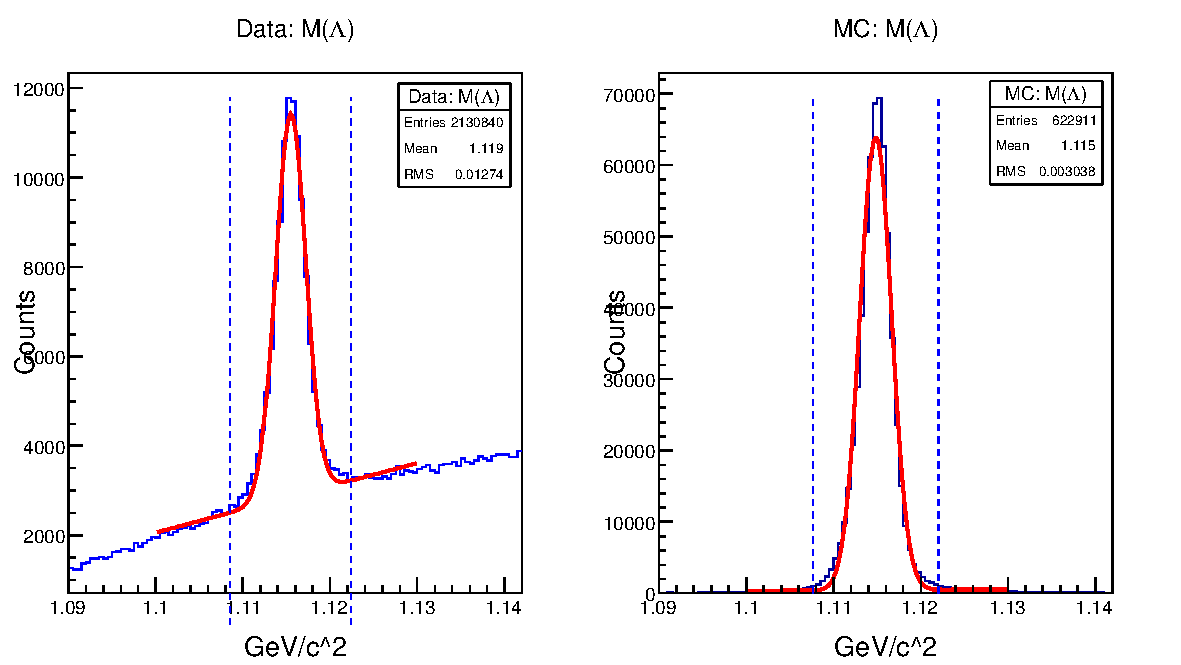
\includegraphics[width=\linewidth]{lambda}
    \caption{Shown is the invariant mass of the $\pi^{-}p$ pair for both the data (left) and simulation (right). The red lines represent a first order polynomial along with a Gaussian fit yielding the centroid for the data (MC) to be 1.1155 (1.1148) GeV and the corresponding $\sigma$ to be $1.73\times 10^{-3}$ ($1.80\times 10^{-3}$) GeV}
        \label{fig:lambdafit}%
\end{figure}

\begin{figure}[h]
    \centering
      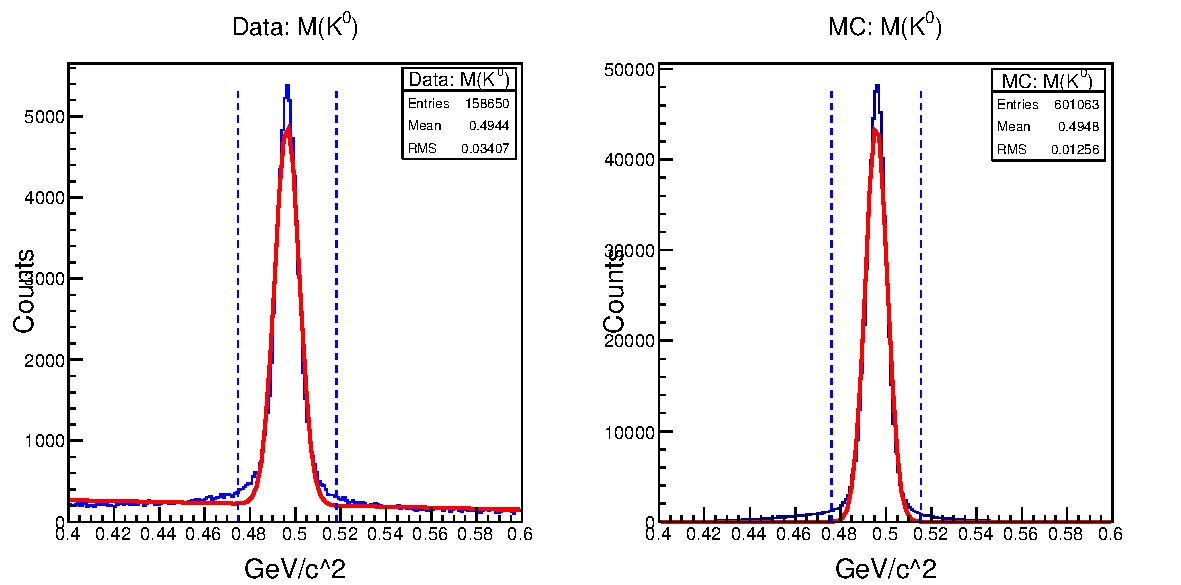
\includegraphics[width=\linewidth]{kaon}
    \caption{Shown is the invariant mass of the $\pi^{+}\pi^{-}$ pair for both the data (left) and simulation (right). The red lines represent a first order polynomial along with a Gaussian fit yielding the centroid for the data (MC) to be 0.4964 (0.4958) GeV and the corresponding $\sigma$ to be $5.44\times 10^{-3}$ ($4.89 \times 10^{-3}$) GeV}
        \label{fig:kaonfit}%
\end{figure}

\subsection{Yield Extraction}
Extraction of the exclusive $\gamma n_{b} \rightarrow K_{s}\Lambda$ events from the sample of $\gamma d \rightarrow \pi^{+}\pi^{-}\pi^{-}pX$ events requires the background contributions to be identified and removed (or accounted for). Also, final-state-interaction events need to be eliminated or strongly suppressed. Previous studies of the reaction of interest\cite{bib:ref6} have shown that the distribution of the missing mass off the kaon, $MM(\gamma n,K)$ (where $n$ is assumed to be at rest), versus the missing mass off $K\Lambda$, $MM(\gamma d,K\Lambda)$, is useful in understanding background contributions from reactions with higher-mass hyperons such as $\Sigma^{0}$ and $\Sigma^{*}$.The events of interest yield a peak in $MM(\gamma n,K)$ at the $\Lambda$ mass.The peak is much wider, compared to $K^{+}\Lambda$ production off the free proton, since the Fermi momentum of the target neutron is not taken into account in the calculation of $MM(\gamma n,K)$. Just this quantity alone is not sufficient to remove background. While the $\Sigma^{0}$ cannot be removed with a simple cut, the $\Sigma^{*}$ contribution can be significantly reduced by removing all events with $MM(\gamma d,K\Lambda) > 1.05$ (Gev/c$^{2}$). This means the $\Sigma^{*}$ signal does not reach underneath the $\Lambda$ signal when looking at a projection onto $MM(\gamma d,K\Lambda)$.
Therefore this quantity was used for the yield extraction as discussed throughout this note.

The distributions in Figure \ref{fig:7} illustrate the clean distributions of the missing mass corresponding to the $\gamma D$ $\longrightarrow K^{0}\Lambda(p)$ and $\gamma D$ $\longrightarrow K^{0}\Sigma(p)$ reactions. The cuts on missing momentum remove most events that would require the associated production of a $\pi^{0}$ (or $\pi^{+}$) such as in the case of the higher-mass hyperons $\Sigma^{*}$ and $\Lambda^{*}$. The yields for both of these reactions can be determined by fitting the both missing mass peaks that remain after the cuts. Both the proton peak (corresponding to the missing mass of the ${K}^{0}\Lambda$) and the proton plus photon peak ($K_{S}\Sigma^{0}$) can be fit to first order with a single Gaussian separately. However, to extract a more reliable yield the fitting of $K_{S}\Sigma^{0}$ can be approached by other means. Understanding the background shapes under the signal was one of the challenges of this analysis. Generated data allowed us to get a very good approximation of the background contributions, and these were used to perform background subtraction as described in the next section. Specifically, the shape of the background was determined by fitting the simulated $K_{S}\Sigma^{0}$ after it was process through the modeled detector. This shape was then the scaled to match the distribution of our actual data. The yields were extracted by the integration of the signal and by fitting the background shapes to the data. 

For full development of the differential cross sections, the data was binned in terms of both photon energy and cos($\theta^{CM}_{K_{s}}$) and their values were then normalized to the photon flux. The normalized yields were then acceptance-corrected from the results of the Monte Carlo simulation. First, the yield correction factor was calculated by studying how many good events are lost as functions of varying the cuts. This will give measure of the systematics. Similarly, the acceptance was calculated using a realistic representation of the CLAS detector in the GEANT simulation.

The final yield is determined after several iterations of corrections to the cuts on the $\delta t$ vs. momentum, track timing, invariant mass and missing momentum. Fiducial cuts of the CLAS detector were made to cut out unreliable events. Corrections to the photon beam energy were already cooked into the data, to account for the sagging of the tagger. Track momentum was also corrected to get a more accurate description of the kinematics. These steps are discussed in detail in the following sections.


\begin{figure}[h]
    \centering
      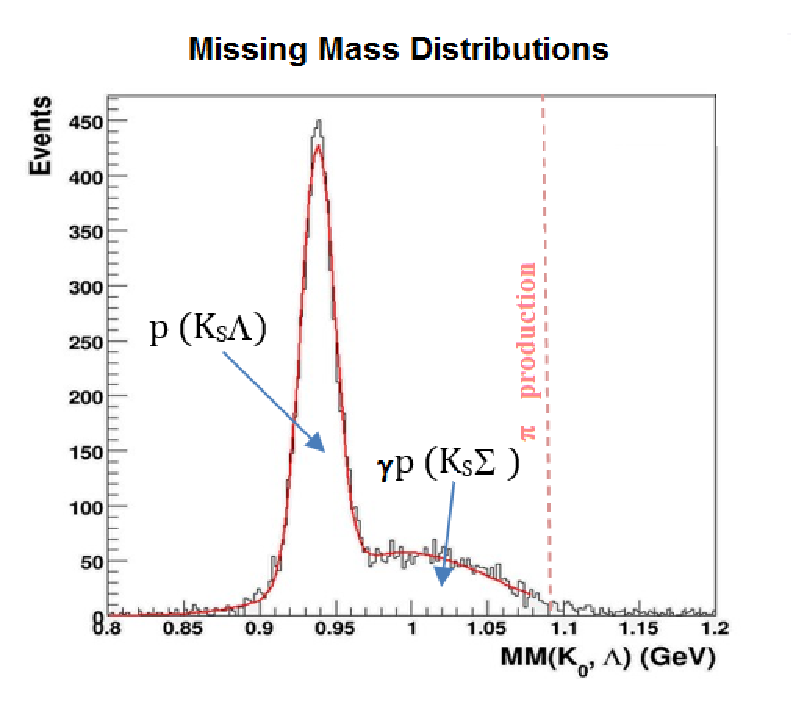
\includegraphics[width=\linewidth, height = 3in, keepaspectratio = true]{MissingMass}
    \caption{The missing mass distribution peaks about the proton mass due to the creation of $K^{0}_{S}\Lambda$. Another distribution can be seen from a missing proton plus photon which is largely associated with the $K^{0}_{S}\Sigma^{0}$. Events with an extra pion including $\Sigma^{*}$ do not contribute to peak associated with $K^{0}_{S}\Lambda$, even if they survived the cuts used in isolating the signal. This is because an extra missing pion would push the missing mass to the right of the red dotted line (shown above). In this figure the $K^{0}_{S}\Sigma^{*}$ was mostly removed with a missing momentum cut.}
        \label{fig:7}%
\end{figure}

\subsection{Background Subtraction}
The reaction of interest is $\gamma n\rightarrow K^{0}\Lambda$. However, to measure this process the decay products of $K^{0}_{S}$ and $\Lambda$ are detected. Therefore the final state particles that are detected are $\pi^{-}\pi^{+}\pi^{-}p$. The four tracks could be produced several different ways. The backgrounds can be attributed to two categories. The first category is a five (or more) track background, where one (or more) tracks were missed by CLAS. The second category of background processes are from a four track background.

\subsection{Five Track Background} \label{sec:fiveparticleback}
By extracting the yield through the missing mass, it is likely that any process producing an extra pion (or other massive particle) is well separated from the spectator proton missing mass measured by $MM(K^{0}\Lambda) = \sqrt{(P_{d}+P_{\gamma} -P_{K^{0}} - P_{\Lambda})^{2}}$. Near the missing mass signal the most prevalent five track background is identified as $\gamma n \rightarrow K^{0}\Sigma^{0} \rightarrow K^{0}\Lambda(\gamma)\rightarrow \pi^{-}\pi^{+}\pi^{-}p(\gamma)$. Nonetheless other background channels were also explored.

\subsubsection{$\gamma n \rightarrow K^{0}\Sigma^{0}$}
The $K^{0}\Sigma^{0}$ background can't be separated from the $K^{0}\Lambda$ signal except through the missing mass as this will still produce a peak at the $\Lambda$ and $K^{0}$ masses. The characteristic shape of this background is explored through simulation. When extracting yield for the $K^{0}\Lambda$ channel a fit to this background shape is used to subtract the $K^{0}\Sigma^{0}$ events. This background combined with simulated $K^{0}\Lambda$ events can represent the data fairly well. Other five track backgrounds that do not produce real $K^{0}$'s or $\Lambda$'s will be significantly reduced by invariant mass cuts and/or be separated from the signal by a large missing mass.

\subsubsection{$\gamma n \rightarrow K^{*}\Lambda$ and $\gamma n \rightarrow K^{0}\Sigma^{*}$}
A comparison of channels was made as a simple study of acceptances. An equal number of events were generated for the $K^{0}\Lambda$ channel and the two lowest energy competing background channels- the $K^{0}\Sigma^{*}$ and K(892)$^{*}\Lambda$  channels. Phase space was used for the event generation. The final results show a very familiar missing mass distribution. There was a negligible contribution of the K(892)$^{*}\Lambda$ channel which reflected the extremely low acceptance. This combined with the improbability that the missing mass is near the spectator proton mass suggests that these channels are not contaminating the dataset. Both the $K^{0}\Lambda$ and $K^{0}\Sigma^{0}$ channels have a distribution ratio very similar to that of the empirical results. It would be reasonable to expect the total cross sections of the $K^{0}\Lambda$ and $K^{0}\Sigma^{0}$ channels to be within one order of magnitude. However, to truly understand the relation between the two reactions, the cross section for both channels would have to have been extracted simultaneously, which was not done in this case in order to avoid using certain assumptions.

\subsection{Four Track Background} \label{sec:fourparticleback}
While the strange channels (such as $K^{0}\Lambda$ and $K^{0}\Sigma^{0}$) are the primary source of our four final state particles events, other processes from nonstrange production mechanisms may contribute to the background. One could imagine that there are several processes to produce this final state. The easiest to consider is the production channel of $\gamma n \rightarrow \rho\Delta^{0}\rightarrow \pi^{-}\pi^{+}\pi^{-}p$.

\subsubsection{$\gamma n \rightarrow \rho\Delta^{0}$}
The neutral delta resonance can also prove a significant contributor to background. In the pairing for a real $\Delta^{0}$ event, the pion pairing method chosen for the analysis would produce a relatively broad distribution about the invariant masses of the $K^{0}$ and $\Lambda$. Likewise if there are other similar background processes, the general trend would be creating a missing mass peak at the value of the proton mass, but would not produce a peak at the kaon or lambda mass. This channel is shown specifically to give an easy example of a real physics event that could create pion background.

\subsubsection{$\gamma n \rightarrow \pi^{-}\pi^{+}\pi^{-}p$}
Regardless of the channel, one would expect scattering events where the final state particles are directly produced from the photon-nucleon interaction. In this case the background from the direct interaction $\gamma n \rightarrow \pi^{-}\pi^{+}\pi^{-}p$ is expected. In the end there are several processes that can produce the final state particles of $\pi^{-}\pi^{+}\pi^{-}p$. This can be used as an advantage when analyzing the background. Because there can be multiple channels contributing to the background, it can be considered as random. This ``random" distribution will result with kinematics filling in the phase space underneath the signal peaks ($K^{0}$ and $\Lambda$). A uniform phase space distribution was generated to model such a background. Although most of the generated phase space events are not in the shown region, the events that are match to the background shape under the $\Lambda$ signal and are linear under the $K^{0}$ signal (after a cut on $M(\Lambda)$) as seen by Figure \ref{fig:lamphase}. To account for this background the sidebands of $K^{0}$ were projected onto the missing mass plane, where by definition this background creates a peak at the spectator proton mass.

This also shows that within the pion background simulation the $K^{0}$ sideband regions produce a missing mass signal that is equal (within statistical fluctuation) to that of the peak region; therefore validating the subtraction method. An estimation of the background contamination within the data is seen. 

\begin{figure}[h]
    \centering
      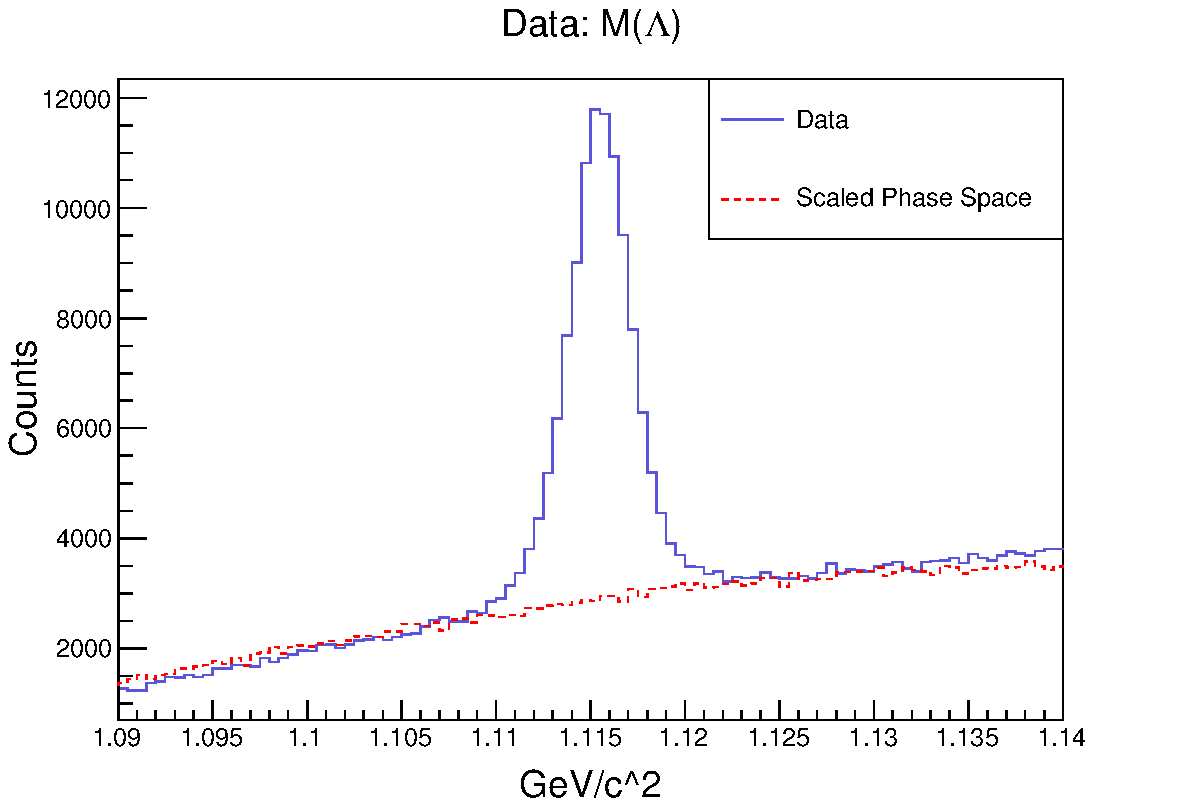
\includegraphics[width=\linewidth, height = 3in, keepaspectratio = true]{lamphase}
    \caption{A uniform phase space distribution was generated to model the background (here shown for the invariant mass of the lambda particle). Although most of the generated phase space events are not in the shown region, the events that are match to the background shape under the $\Lambda$ signal and are linear under the $K^{0}$ signal (after a cut on $M(\Lambda)$) as seen by Figure \ref{fig:lamphase}. To account for this background the sidebands of $K^{0}$ were projected onto the missing mass plane, where by definition this background creates a peak at the spectator proton mass}
        \label{fig:lamphase}%
\end{figure}

\subsection{Photon Flux}
An important part of measuring any cross section is the number of incident photons on the target. This quantity is measured and recorded separate data files and requires separate processing. Events without the photon flux records were dropped from analysis. Analysis was also performed on the consistency of the flux files which allowed an estimate of how consistent the run was within itself. This was applied into the uncertainty of cross section per bin. 

\subsection{Monte Carlo Simulation}
Monte Carlo simulation is used to determine the true acceptances in the CLAS detector. In principle the CLAS detector provides $4\pi$ acceptance, but in reality, the detector has several ``blind'' spots and low regions of efficiency. The simulation only generates the $K_{S}\Lambda$ or $K_{S}\Sigma$ events separately.
Their missing masses are then later approximated in proportions with respect to the real data. After event generation, the simulated particles are sent through the model of the detector with the GSIM package. The results are then filtered through additional routines to make further corrections to the real detector efficiencies.  

\subsubsection{Event Generation}
For this study, \textit{fsgen} (a FORTRAN code which uses the PYTHIA framework) was used for the event generator. For practical reasons, \textit{fsgen} uses pre-generated ``Lund" tables to begin the event generation. These tables hold the decay tables for many of the hadrons. The decay or scatter of the excited nucleon is not performed with \textit{fsgen}. Instead, the event generation begins with the section of photon energy. With this energy, the Fermi momentum was determined using the Bonn distribution and the center-of-mass energy, which determined the momentum distribution. The Bonn potential is based on the exchange of mesons between the nucleons\cite{ref13}. In its simplest form (before the Fourier transform), the potential can be written as;

\vspace{5mm} %5mm vertical space
\begin{equation} 
V^{loc}_p=-\frac{g^2}{4M^2}\frac{\left({{\mathbf s}}_{{\mathbf 1}}{\mathbf k}\right)\left({{\mathbf s}}_{{\mathbf 2}}{\mathbf k}\right)}{k^2+m^2_p}  ,  \label{EQ3}      
\end{equation} 
\vspace{5mm} %5mm vertical space

\noindent Where g is the coupling constant for the pN interaction, M is the mass of the nucleon, $\sigma{}_{i}$ are the Pauli spin matrices, and k is the difference of the relative 4-momenta in their initial and final states. The code then uses two factors to calculate the angular distribution of the decay/scatter hadron- a user defined function for the cosine theta and a defined t-slope value, where the t-slope is b in the differential cross section:

\vspace{5mm} %5mm vertical space
\begin{equation} 
\frac{ds}{dt}=s_{0}e^{-bt} .     \label{EQ4}  
\end{equation} 
\vspace{5mm} %5mm vertical space

\noindent Here s${}_{0}$ is the amplitude of the cross section and t is the squared 4-momentum transfer. The t-slope can be varied to a user defined method.

\FloatBarrier
\subsubsection{Event Processing}
Once the quality of the generated events has been verified, they are passed to the GSIM code. The GSIM package uses GEANT4 to propagate these particles through a simulated CLAS system. These GSIM parameters were taken from P. Mattione in the files ``gsim\_53600.ffread" and ``gsim\_cook\_g13.tcl". The short-lived K$\Sigma$ and $\Lambda$ particles are decayed during this stage of the simulation.
Most of the generated neutral particles decay before they reach the start counter.
The trajectories and energies of the final-state particles are recorded into the data banks as individual measurements of subdetector systems.
The simulated BOS files have the same structure as the real BOS files, but have additional MC banks. These additional banks keep the generated information on each track.
%The MCTK bank stores the track information for the neutral particles in addition to the final state tracks.
%The originating vertices for each track are stored in the MCVX bank.
Before these files are cooked and analyzed it is important to first correct for the detector inefficiencies by running the \textit{gpp} package.

The \textit{gpp} code serves two primary purposes- it modifies the tracks to represent the inefficiencies in the current CLAS detector system and it can smear the track's path through the drift chambers to better model the uncertainty of detectors as seen in the experimental data. It also smears the time of the event photon. 

\subsection{Uncertainties}
Systematic uncertainties were determined for each portion of the experiment. This includes errors in target and detector geometries and effects of event selection and cuts. These contributions can be seen in Table \ref{tab:sysuncert}. Most fitting and sector dependent uncertianities were compiled per bin. The propogation of systemmatic errors were combined in quadrature with the total statistical uncertianties. The largest uncertianties were associated with forward angles, where a blind spot exists from the detector geometry, and at backward angles, where statistics and detector efficiencies are poor.  

\begin{table}[h]
\centering
\caption{Summary of the systematic effects, estimating a total average point-to-point uncertainty.}
\label{tab:sysuncert}
\begin{tabular}{|c|c|}
\hline
{\bf Investigated Cut} & {\bf Systematic Uncertainty} \\ \hline
\multicolumn{2}{|c|}{{\bf Luminosity} } \\ \hline
Flux Consistency                  &    2.6-7.0\%    \\ \hline
Target Density                    &    0.11\%    \\ \hline
Target Length                     &    0.3\%    \\ \hline
\multicolumn{2}{|c|}{{\bf Acceptance} } \\ \hline
Yield By Sector                   &   1.6\% - 1.9\%    \\ \hline
Sector Dependence                 &   2.0\%    \\ \hline
Simulation Weighting              &   1.0\%    \\ \hline
\multicolumn{2}{|c|}{{\bf Final State Identification} } \\ \hline
PID                               &   1.1\%    \\ \hline
Multi-Track rejection             &   0.3\%    \\ \hline
Photon Timing                     &   1.4\%    \\ \hline
%Photon Multiplicity               &  Section \ref{sec:photselectcut}  &   2.8\%    \\ \hline
Pion Pairing                      &   1.0\%    \\ \hline
$M(\Lambda)$                      &   0.3\%    \\ \hline
$M(K^{0})$                        &   1.6\%    \\ \hline
Missing Momentum                  &   1.0\%    \\ \hline
\multicolumn{2}{|c|}{{\bf Yield Extraction} } \\ \hline
Bin Width                         &   .02\% - 0.67\%    \\ \hline
$\Sigma^{0}$ Background Function  &   .03\% - 10.74\%    \\ \hline
$\Sigma^{0}$ Background Mom. Cor. &   3.5\%    \\ \hline 
\multicolumn{2}{|c|}{{\bf CLAS} } \\ \hline
Fiducial Cuts                     &   2.5\%    \\ \hline
\multicolumn{2}{|c|}{{\bf Branching Ratios} } \\ \hline
$K^{0}\rightarrow K^{0}_{S}$           &   -    \\ \hline
$K^{0}_{S}\rightarrow \pi^{+}\pi^{-}$  &   0.05\%  \\ \hline
$\Lambda \rightarrow \pi^{-}p$         &   0.5\%    \\ \hline
\multicolumn{1}{|c|}{{\bf Total} }   &   {\bf 6.41\% - 14.15\%}    \\ \hline
\end{tabular}
\end{table}


%_____________________________EXPERIMENTAL_RESULTS________________________

\section{Experimental Results}
\subsection{Model of the $K^{0}\Lambda$ Differential Cross Section}
Several models have been developed for kaon photoproduction channels (fig. \ref{fig:theoryResonance}). However while most show consistency (particularly the proton interactions with SAPHIR data), the $K^{0}\Lambda$ channel shows and order of magnitude difference. The 1999 model for the $K^{0}\Lambda$ cross section is shown in fig. \ref{fig:theoryResonance} as a solid line. The older 1997 model is presented by the dashed line\cite{bib:model2}

Another model was developed by D. Drechsel and L. Tiator for kaon differential cross sections for unpolarized target and without recoil polarization\cite{bib:XSectionTheory}. They review the formalism for polarization degrees of freedom for pion threshold experiments, and present the multipole decomposition of the various response functions. The model can be written as;

\vspace{5mm} %5mm vertical space
\begin{equation} 
\frac{d\sigma}{d\Omega_{f}dE_{f}d\Omega}=\Gamma \frac{d\sigma_{\nu}}{d\Omega},
\label{EQ4} 
\end{equation} 
\vspace{5mm} %5mm vertical space

where where the flux of the virtual photon field is, 

\vspace{5mm} %5mm vertical space
\begin{equation} 
\Gamma = \frac{\alpha }{2\pi^{2}}\frac{E_{f}}{E_{i}}\frac{k_{\gamma}}{Q^{2}}\frac{1}{1-\varepsilon},
\label{EQ5} 
\end{equation} 
\vspace{5mm} %5mm vertical space

and

\vspace{5mm} %5mm vertical space
\begin{equation} 
\begin{split}
\frac{d\sigma_{\nu}}{d\Omega}= \frac{d\sigma_{T}}{d\Omega} + \varepsilon \frac{d\sigma_{L}}{d\Omega} + \sqrt{2\varepsilon\left ( 1 - \varepsilon \right )}\frac{d\sigma_{LT}}{d\Omega}cos\phi  \\  
+ \varepsilon \frac{d\sigma_{TT}}{d\Omega}cos2\phi  + h \sqrt{2\varepsilon\left ( 1 - \varepsilon \right )}\frac{d\sigma_{LT'}}{d\Omega}sin\phi.
\label{EQ6}  
\end{split}                                                
\end{equation} 
\vspace{5mm} %5mm vertical space

\begin{figure}[t]
    \centering
      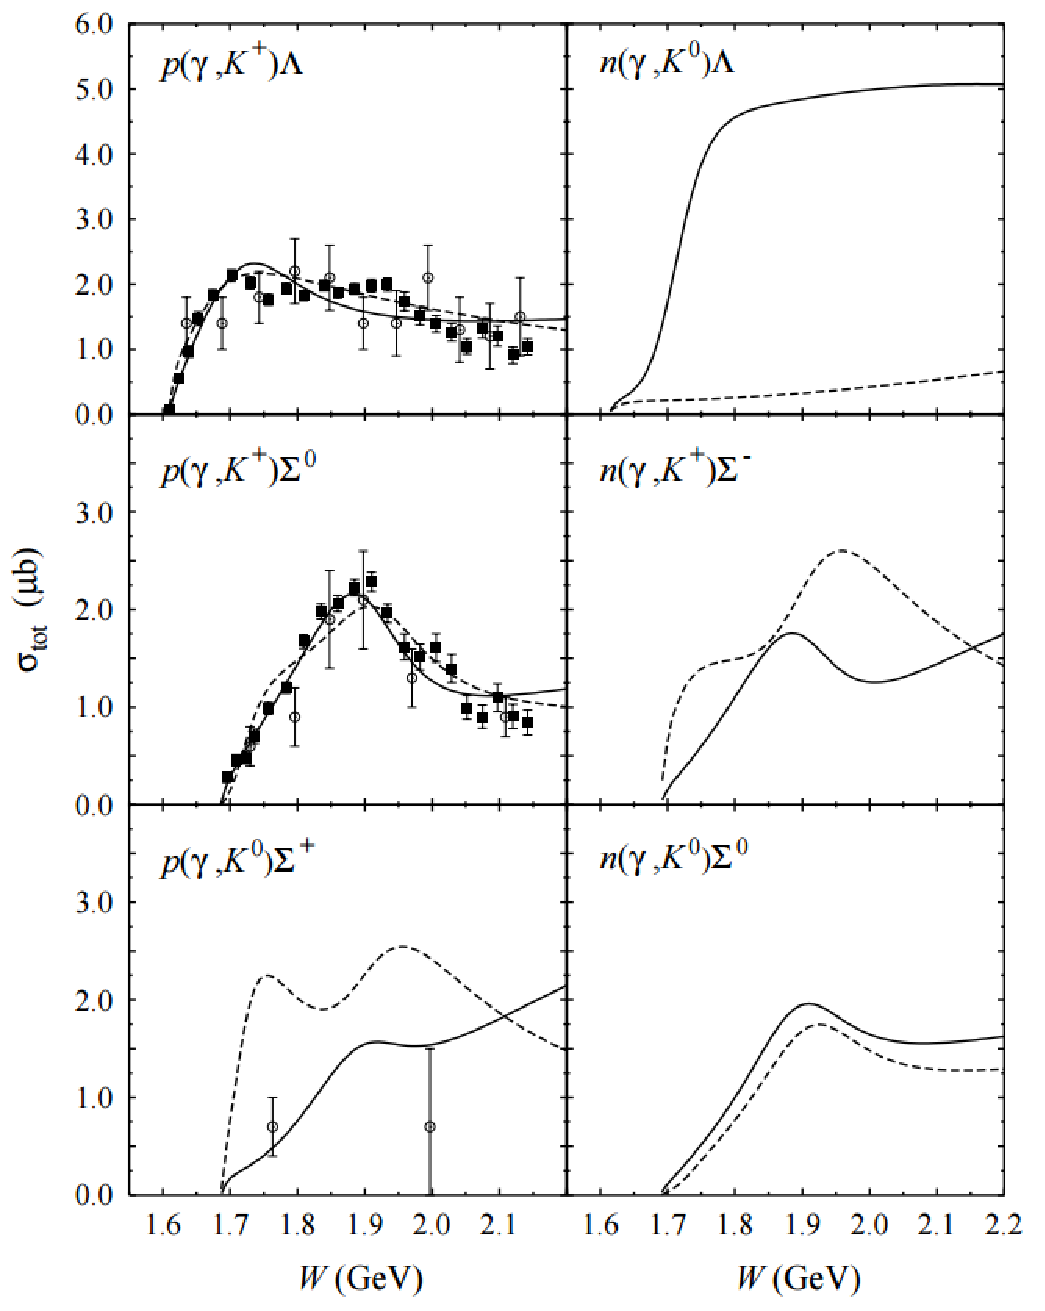
\includegraphics[width=\linewidth]{theoryResonance}
    \caption{Some of the possible kaon photoproduction channels compared to  experimental data (figure from H. Yamamura, et al.\cite{bib:model1}). The solid curve is is the later 1999 model and the older 1997 model is presented by the dashed line\cite{bib:model2}. SAPHIR’s data is plotted as the solid squares, while the older data is denoted with dots.}
        \label{fig:theoryResonance}%
\end{figure}

The first two terms of eq. \ref{EQ6} corrispond to the transverse (T) and Longitudinal (L) structure functions. The third and fifth terms describe the transvers-longitudinal interferences (TL and TL'), which are dependent on the cosine and sine of the azmuthal angle.  The forth term relates to the transverse-transverse interference (TT) while the last term (TT) can only be observed by target or recoil polarizations. 

\subsection{$K^{0}\Lambda$ Differential Cross Section} \label{sec:diffcross}
The differential cross section for the $\gamma n \rightarrow K_{s}\Lambda$ reaction can be rewritten as: 

\vspace{5mm} %5mm vertical space
\begin{equation} 
\begin{split}
\frac{d\sigma}{dcos\theta^{CM}_{K_{S}}}=\frac{A_{target}}{\rho\ell N_A}\frac{1}{\Delta cos\theta^{CM}_{K_{S}}}\frac{Y\left(\sqrt{s},\theta^{CM}_{Ks}\ \right)}{\phi\left(\sqrt{s}\right)}\frac{Y_{CF}}{\alpha\left(\sqrt{s},\theta^{CM}_{K_{S}}\right)}   \\
\frac{\Gamma_{K^{0}}}{\Gamma_{K^{0}}\rightarrow K_{S}}\frac{\Gamma_{K_{S}}}{\Gamma_{K_{S}}\rightarrow\pi^+\pi^-}\frac{\Gamma_{\Lambda }}{\Gamma_{\Lambda}\rightarrow p\pi^-},
\label{EQ12}  
\end{split}                                                
\end{equation} 
\vspace{5mm} %5mm vertical space

\noindent where $A_{target}$ is the atomic weight of the target, $rho$ is the density of the target, $\ell$ is the length of the target, $N_{A}$ is Avogadro's number, $\Delta\cos({\theta}^{CM}_{Ks})$ is the bin width of the cosine theta, $Y$($s$ ,${\theta}^{CM}_{Ks}$) is the yield, $\phi$ is the photon flux, $Y_{CF}$ is the yield correction factor, $\alpha$ is the acceptance used, and the inverse branching ratios of the decay channels for the neutral hadrons are represented by $\Gamma_{K_{S}}/(\Gamma_{K_{S}}\rightarrow\pi^{+}\pi^{-})$, $\Gamma_{K_{S}}/(\Gamma_{K_{S}}\rightarrow\pi^{+}\pi^{-})$  and $\Gamma_{\Lambda}/(\Gamma_{\Lambda}\rightarrow p\pi^{-})$.

Using the g13 data set, figure \ref{fig:XScosineTheta} shows the differential cross section of the  $\gamma n \rightarrow K_{s}\Lambda$ reaction with respect to $\cos(\theta^{K^{0}}_{CM})$ for 1 GeV photon energy bins between 0.9 to 2.5 GeV. In figure \ref{fig:XSenergyW},  the cross section is rebinned by the center-of-mass energy for various $\cos(\theta^{K^{0}})$ bins for both g10 and g13 data sets.  The approximated Drechsel and Tiator is also shown, assuming no contribution from the K$_{1}(1270)$, S$_{31}$(1900) and P$_{31}$(1910). Close agreement is seen between the two experiments, with some discrepancies in the forward bin-- 0.7 to 0.8 $\cos(\theta^{K^{0}})$.

\begin{figure*}[h]
    \centering
      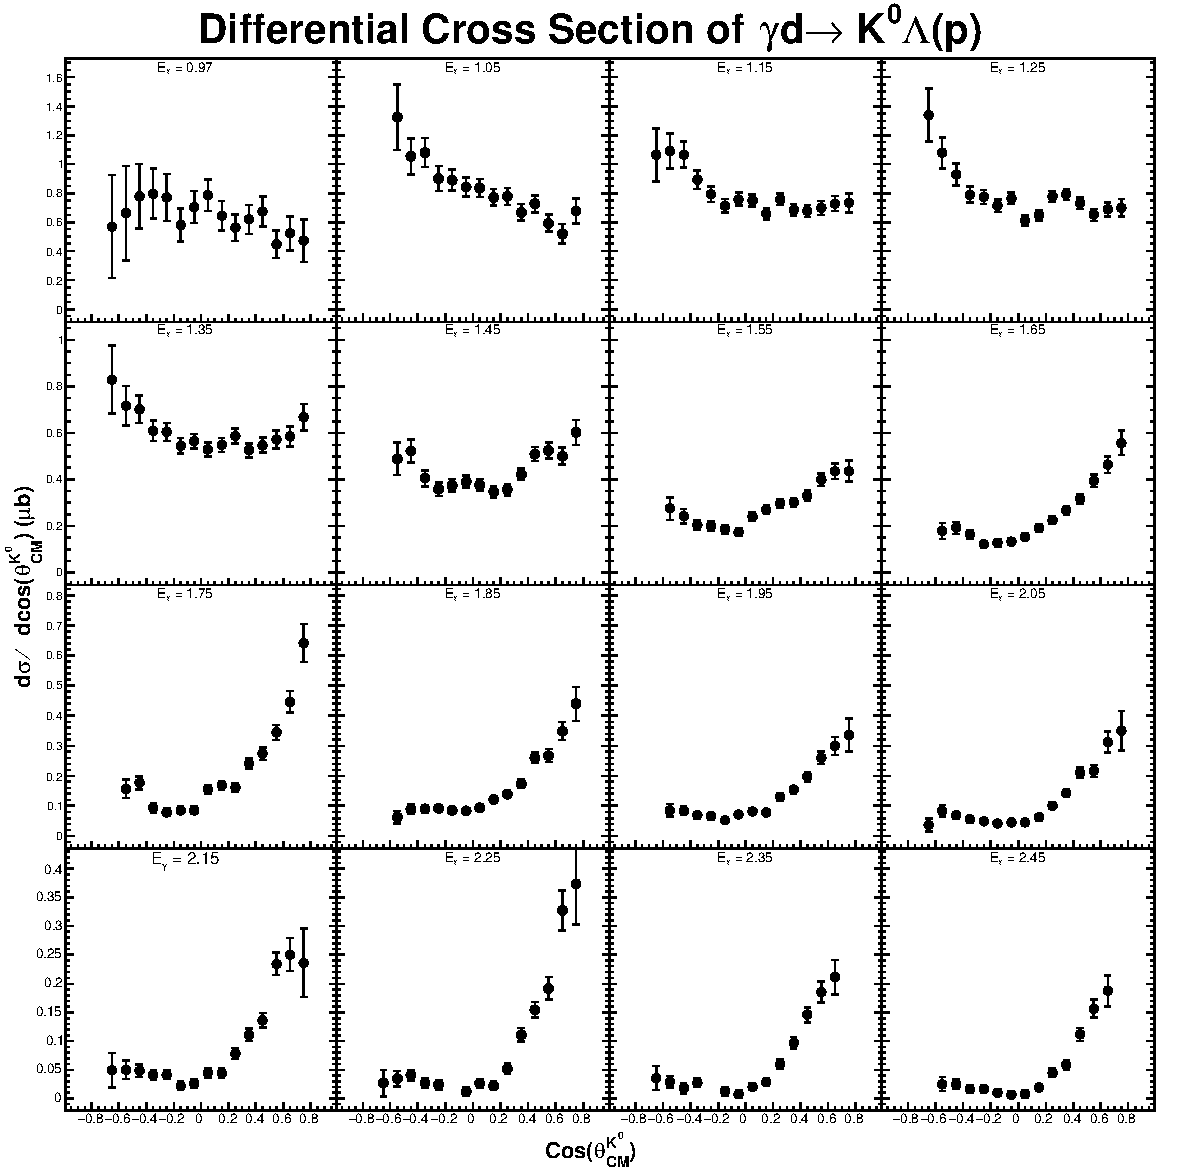
\includegraphics[width=5.5in, keepaspectratio=true]{crossSection}
    \caption{The differential cross sections in bins of $\cos(\theta^{K^{0}}_{CM})$ for each beam energy.}
        \label{fig:XScosineTheta}%
\end{figure*}

\begin{figure*}[h]
    \centering
      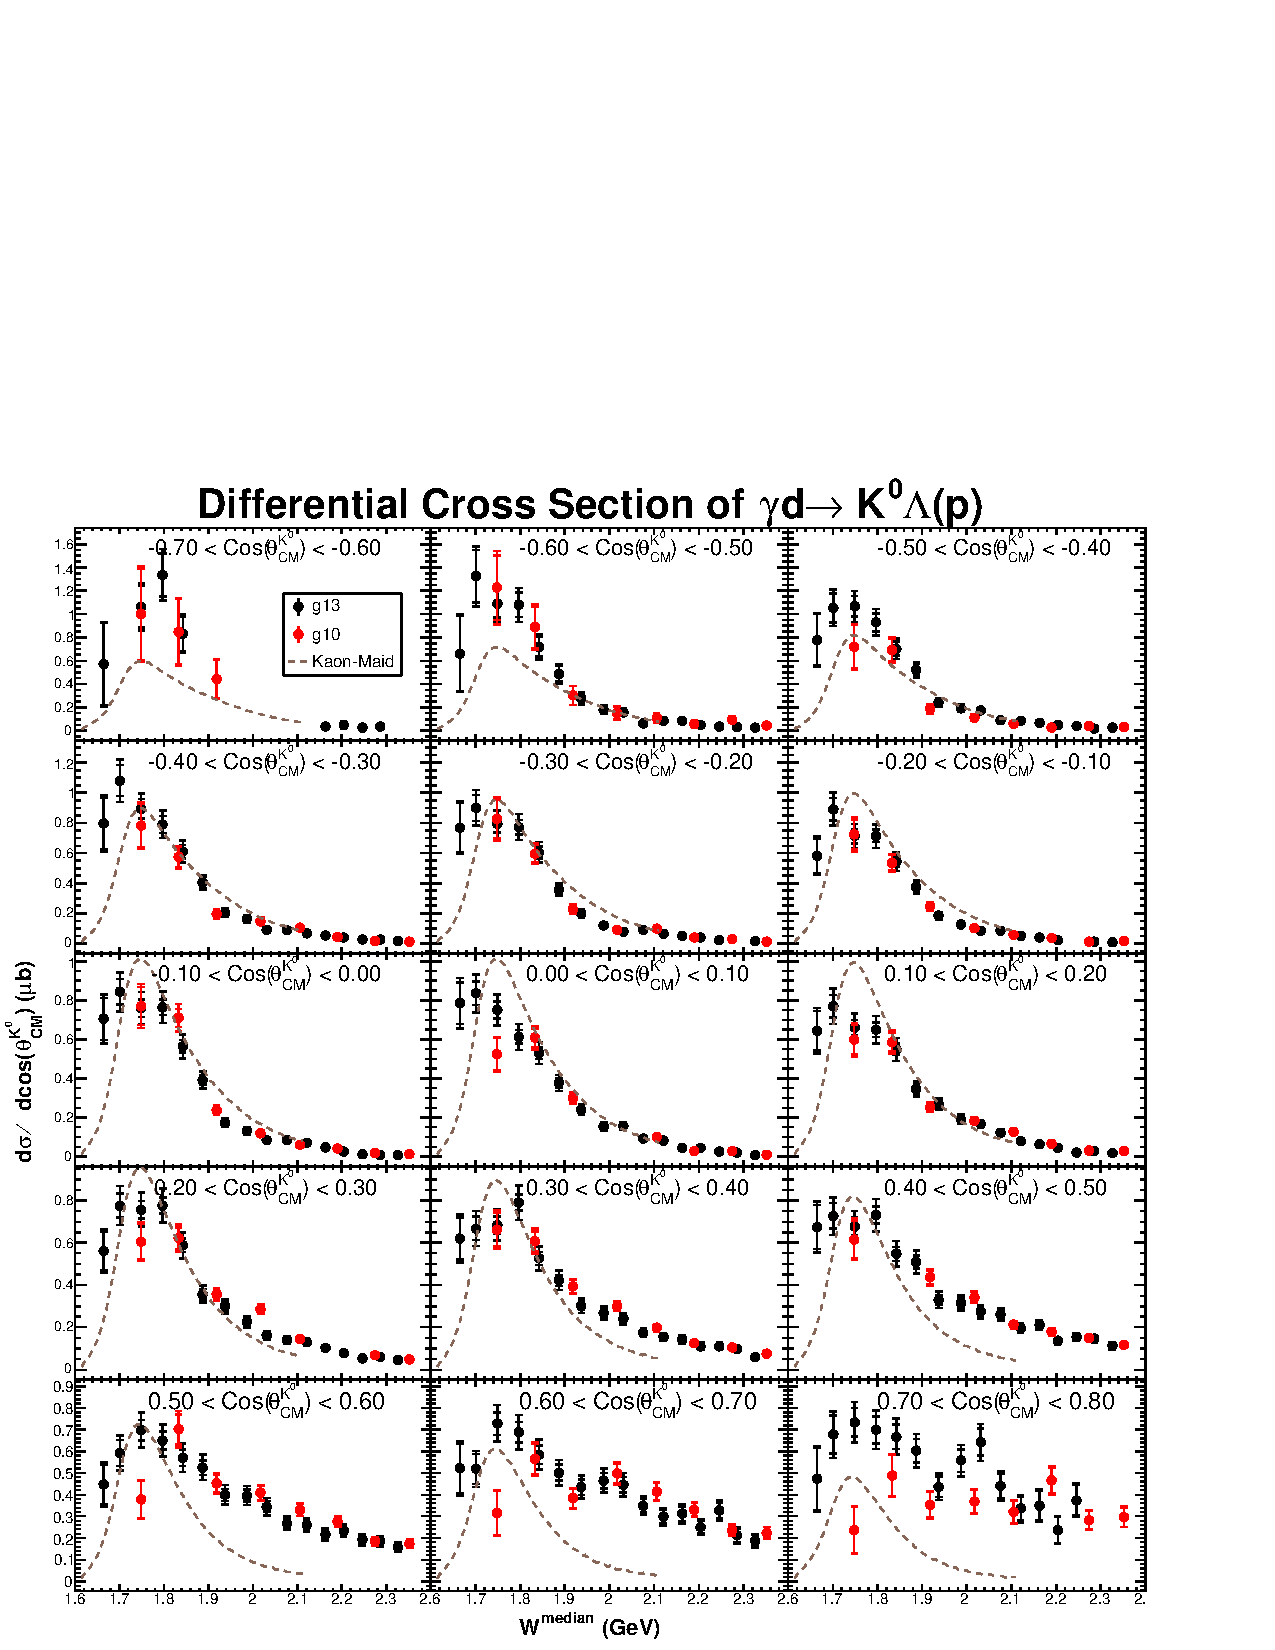
\includegraphics[width=6in, keepaspectratio=true]{crossSectionAngleWK1offKSoff}
    \caption{The differential cross sections in bins of $W$ (GeV) for each $\cos(\theta^{K^{0}}_{CM})$, using the g13 data set (seen by the black points).}
        \label{fig:XSenergyW}%
\end{figure*}

\FloatBarrier
\subsection{Total Cross Section}
The total cross section can be found by integrating over all $\cos(\theta^{K^{0}}_{CM})$ of the differential cross section. This has two sources of uncertainty, the uncertainty of the fit to the points, as well as uncertainty associated with the absence of points at extreme angles. The absence of these points although makes this estimation more difficult, it does not prevent a reasonable estimation of the total cross section to be obtained. Assuming specific functions can fit the data well and have realistic behaviors near the forward and backward angles, the fits could be used for to extrapolate to these angles. Since many functions could fit the majority of the data well, the uncertainty in the extrapolation can be approximated by utilizing several well fitting functions and using the variation in results as an added uncertainty. Figure \ref{fig:CrossfitperE} demonstrates several fits to the data with the integrated cross sections shown in Figure \ref{fig:totcrossfit}. Using the third order Legendre Polynomial as the base fit, the total cross section is shown in Figure \ref{fig:totcross}.

\begin{figure}[t]
    \centering
      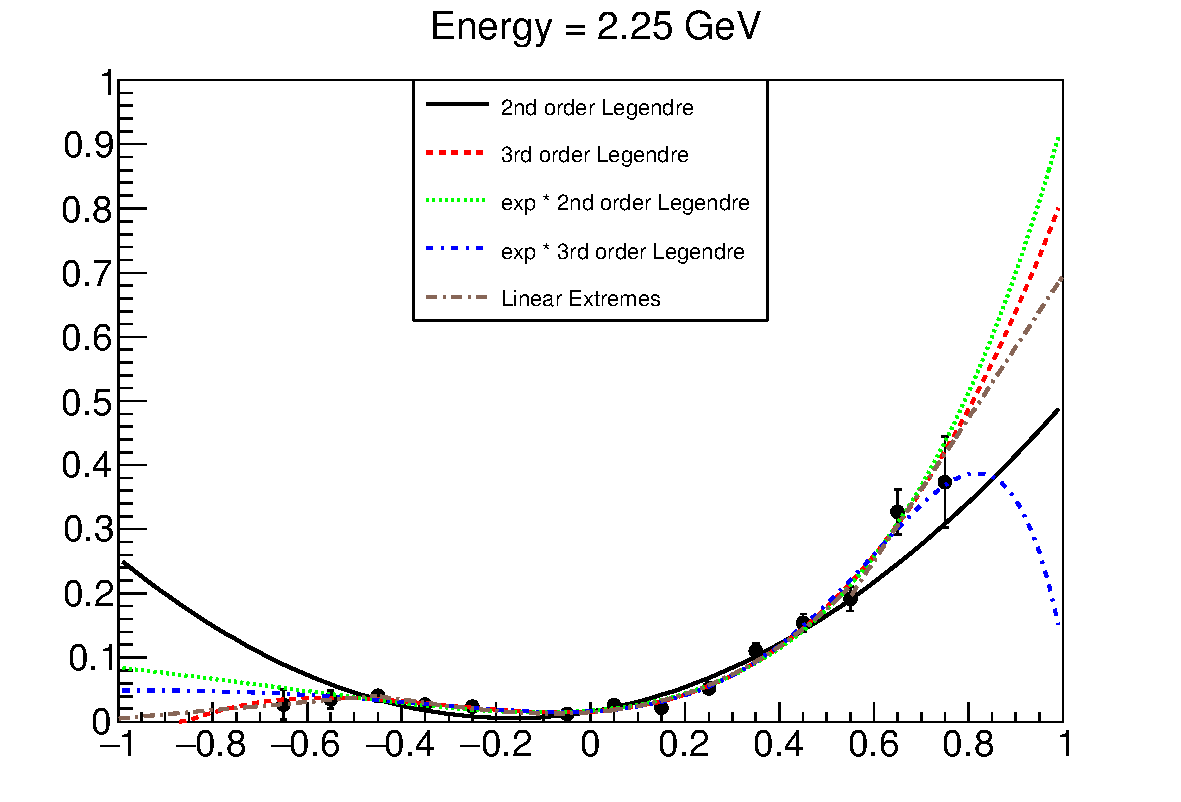
\includegraphics[width=\linewidth]{CrossfitperE}
    \caption{Different fits of the differential cross sections using...}
        \label{fig:CrossfitperE}%
\end{figure}

\begin{figure}[t]
    \centering
      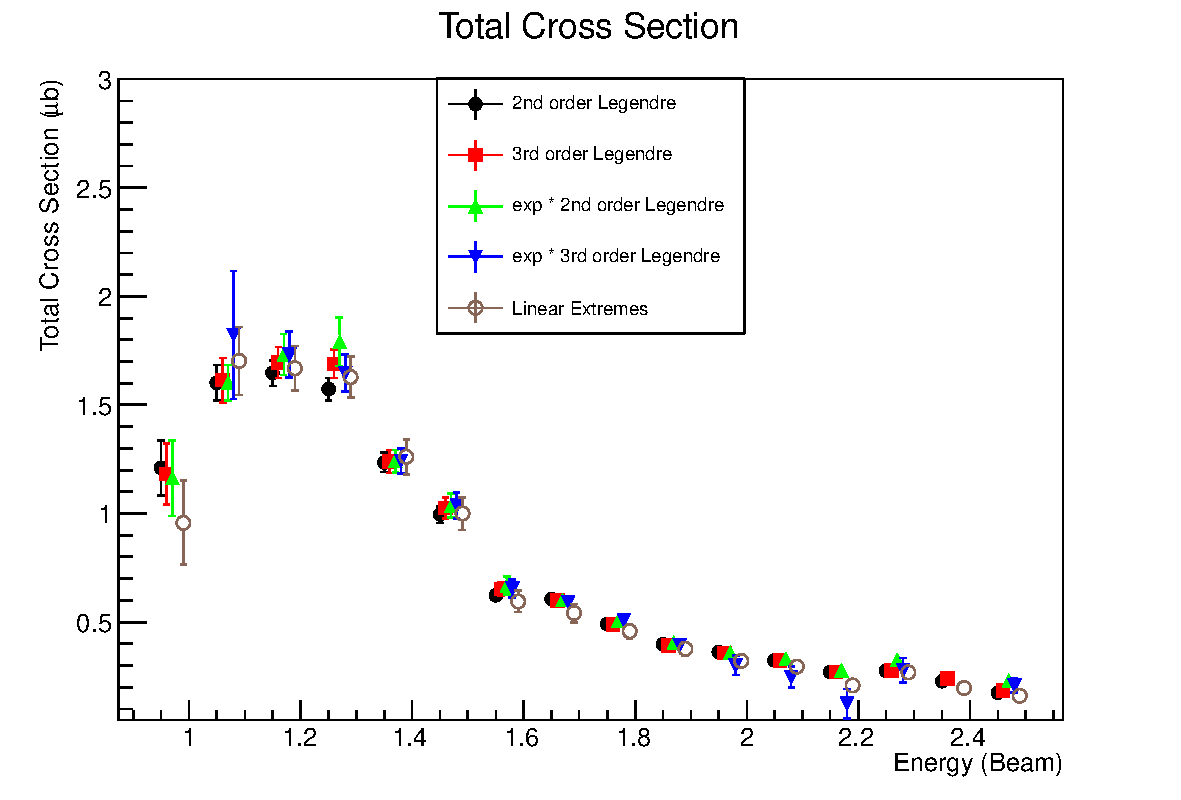
\includegraphics[width=\linewidth]{totcrossfits}
    \caption{Fits of the differential cross sections using...}
        \label{fig:totcrossfit}%
\end{figure}

\begin{figure}[t]
    \centering
      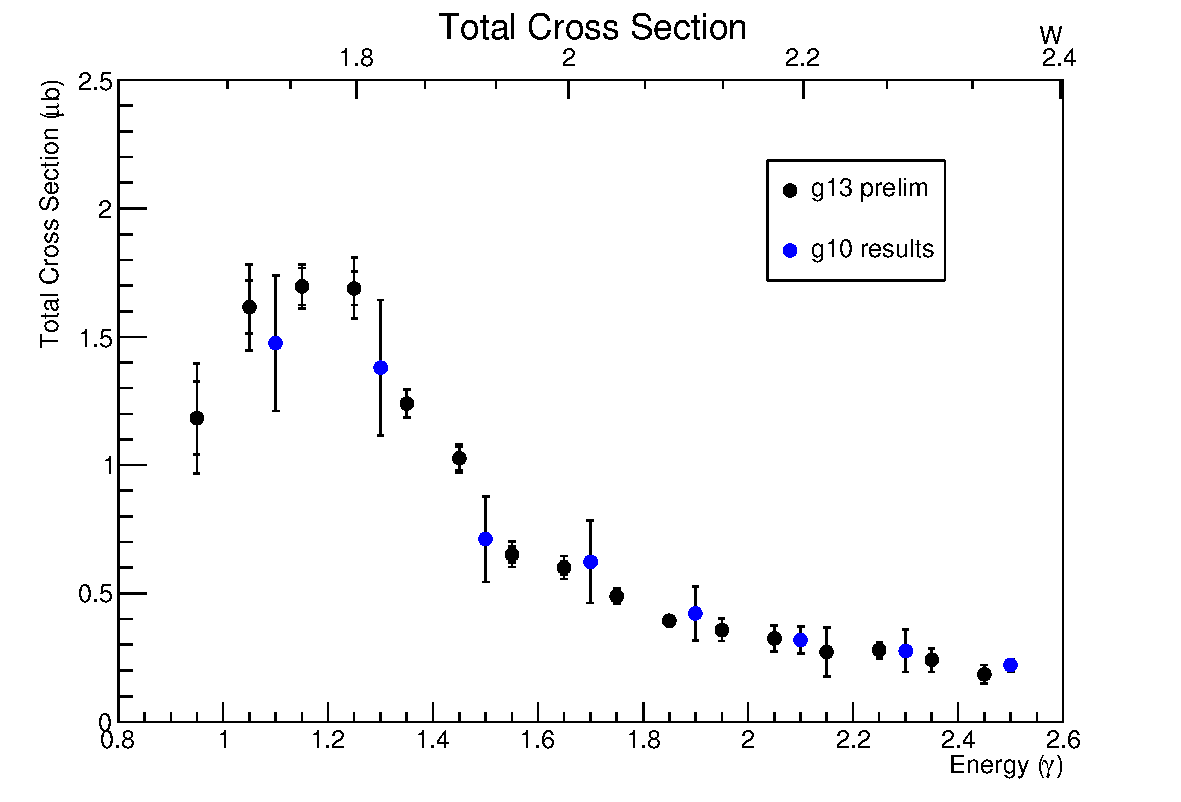
\includegraphics[width=\linewidth]{totcross}
    \caption{The total cross section results from both g13 and g10 experiments.}
        \label{fig:totcross}%
\end{figure}

%_____________________________CONCLUSIONS________________________
\section{Conclusions}
The cross sections extracted from both the g10 and g13 datasets are in very close agreement, with its greatest deviation in the last cosine theta bin ($0.7 < \cos(\theta^{K^{0}}_{CM}) < 0.8$). While the g10 and g13 energy bins were not the same, their distributions show the same evidence of excess cross section at $W \sim 1.7$ and $1.8$ GeV.


%Not sure the best way to conclude. The 1.7 is in agreement with both SAPHIR and McNabb, but the 1.8 is clearly not in agreement with the K+ channel.  It is possible k0 is coupling more to the third P13 than the third D13. Dunno.


%________________________________________________________
%appendix on Cross section numbers
\FloatBarrier
\appendix
\section{Table of Cross Sections}


\begin{table}[h]
\centering
\caption{Total Cross Section}
\label{tab:diffcross1}
\begin{tabular}{|c|c|c|c|c|}
\hline
 {\bf Energy} &  {\bf $d\sigma(E_{\gamma})$ ($\mu b$)} & {\bf Stat. Uncert($\mu b$)} & {\bf Syst. Uncert($\mu b$)} \\ \hline
 0.95 &  1.207  &  0.190  &  0.035   \\ \hline
 1.05 &  1.827  &  0.156  &  0.249   \\ \hline
 1.15 &  1.810  &  0.083  &  0.082   \\ \hline
 1.25 &  1.854  &  0.075  &  0.170   \\ \hline
 1.35 &  1.329  &  0.061  &  0.014   \\ \hline
 1.45 &  1.060  &  0.058  &  0.059   \\ \hline
 1.55 &  0.698  &  0.040  &  0.062   \\ \hline
 1.65 &  0.634  &  0.032  &  0.038   \\ \hline
 1.75 &  0.564  &  0.028  &  0.015   \\ \hline
 1.85 &  0.384  &  0.022  &  0.096   \\ \hline
 1.95 &  0.361  &  0.021  &  0.044   \\ \hline
 2.05 &  0.330  &  0.016  &  0.077   \\ \hline
 2.15 &  0.273  &  0.015  &  0.056   \\ \hline
 2.25 &  0.277  &  0.015  &  0.039   \\ \hline
 2.35 &  0.238  &  0.014  &  0.047   \\ \hline
 2.45 &  0.195  &  0.014  &  0.028   \\ \hline
\end{tabular}
\end{table}



%_____________________________REFERENCES________________________
\begin{thebibliography}{5}
\bibitem{bib:ref1a}
        R.Koniuk and N. Isgur,
        Phys. Rev. D 21, 1868 (1980).
        
\bibitem{bib:ref1b}
        S. Capstick and W. Roberts,
        Phys. Rev. D 58, 074011 (1998).
        
\bibitem{bib:ref1c}       
		T.Mart, C. Bennhold, and C.E. Hyde-Wright,
		Phys. Rev. C 51, 1074(R) (1995).

\bibitem{bib:model1}       
		H. Yamamura, et. al.,
		Phys. Rev. C 61, 014001 (1999).

\bibitem{bib:model2}       
		C. Bennhold,et. al.,
		{\em Proceedings of the CEBAF/INT Workshop on N* Physics}		
		World Scientific, Scingapore, p 1676 (1999).		

\bibitem{bib:ref1d}
		S. Eidelman, et al., 
		Phys. Lett. B592, 1 (2004).

\bibitem{bib:ref1e}
		M.Q. Tran,
		Phys. Lett. B445, 20 (1998).

\bibitem{bib:ref1f}
		K.H. Glander, et al., 
		Eur. Phys. J. A19, 251 (2004)

\bibitem{bib:ref1g}
		J.W.C. McNabb, et al., 
		Phys. Rev. C 69, 042201 (2004).

\bibitem{bib:ref1h}
		R.Bradford, et al., 
		Phys. Rev. C73, 035202 (2006).
		
\bibitem{bib:ref1i}
        M.E. McCracken,
        {\em A Study of $K^{+}\Lambda$ Photoproduction in the CLAS g11a Dataset: Differential Cross Section, recoil Polarization and a Partial Wave Analysis},
        Doctoral dissertation, Carnegie Mellon University (2008).

\bibitem{bib:ref2}
        K. Livingston,
        Nucl. Instr. and Meth.
        A: 603, 205 (2009). 

\bibitem{bib:ref3}
        D. I. Sober et al.
        The CLAS Collaboration,
        Nucl. Instr. and Meth.:
        A 440, 263 (2000). 

\bibitem{bib:ref4}
        Y. G. Sharabian et al.
        The CLAS Collaboration,
        Nucl. Instr. and Meth.
        A 556, 246 (2006). 

\bibitem{bib:ref5}
        M. Amarian, et al.,
        {\em The CLAS forward electromagnetic calorimeter}, (CLAS),
        Nucl. Instr. and Meth.
        A 460, 239-265(2001).

\bibitem{bib:pdgKshort}       
        K.A. Olive et al. 
        Particle Data Group), Chin. Phys. C38, 090001 (2014) 	 
        URL: http://pdg.lbl.gov)

\bibitem{bib:pdgLambda}
		C. Amsler et al. 
		(Particle Data Group), PL B667, 1 (2008) 
		(URL: http://pdg.lbl.gov)   
        
\bibitem{bib:ref5b}
		W. Chen, et al., 
		A Measurement of the Differential Cross Section for the Reaction$\gamma n \longrightarrow \pi^{-}p$ from Deuterium,
		Phys. Rev. Lett. 103, 012301 (2009).

\bibitem{bib:ref6}
        P. Nadel-Turonski, et al.,
        Jefferson Lab PAC30 Proposal: PR-06-103 (2006). 

\bibitem{bib:ref9}
        E. Pasyuk,
        {\em Energy loss corrections for charged particles in CLAS},
        CLAS-Note 2007-016 (2007).

\bibitem{bib:g13studies}
        P. Mattione,
        \emph{g13 systematic studies},
        note on the systematics of g13.

\bibitem{ref13}
        R. Machleidt,
        {\em The high-precision charge-dependent Bonn nucleon-nucleon potential (CD-Bonn)},
        University of Idaho, arXiv:nucl-th/0006014v1, (2008).

\bibitem{bib:fluxdeter}
        J. Ball and E. Pasyuk,
        \emph{Photon Flux Determination Through Sampling of ``out-of-time" Hits with the Hall B Photon Tagger},
        J. Ball and E. Pasyuk,
        CLAS-Note 2005-002.
        
\bibitem{bib:XSectionTheory}        
        D. Drechsel and L. Tiator, J. Phys. G 18 (1992) 449-497.
        {\em Threshold Pion Photoproduction on Nucleons}, 
        (URL: http://portal.kph.uni-mainz.de/MAID//kaon/kaon-observ.html)

\end{thebibliography}

\end{document}



